\subsubsection{General type refrigerant control volume state equation}
Many of the components in a refrigeration cycle will be based on equations of similar structure. They will generally express the change in mass inside the control volume and/or the specific enthalpy out of the control volume. These can be constructed from the mass conservation equation and the steady state energy balance equation of the control volume. The energy balance equations are modelled as steady state algebraic equations. This lowers accurracy but reduces complexity of the models.

\textbf{Mass conservation equation} \\
\begin{equation} \label{eq:GeneralTypeControlVol_MassConservation}
	\frac{dM}{dt} = \dot{m}_{in}(t) - \dot{m}_{out}(t)
\end{equation}

where
\begin{center}
	\begin{tabular}{l p{8cm} l}
		$\frac{dM}{dt}$ 	& Change in mass inside control volume & [\si{kg}/\si{s}]\\
		$\dot{m_{in}}$ 		& Mass flow of refrigerant into control volume & [\si{kg}/\si{s}]\\
		$\dot{m_{out}}$ 	& Mass flow out of control volume & [\si{kg}/\si{s}]\\
	\end{tabular}
\end{center}

\textbf{Energy balance equation}
\begin{equation}
	h_{out} = h_{in} + \frac{Q_{in}}{\dot{m}_{in}}
\end{equation}

where
\begin{center}
	\begin{tabular}{l p{8cm} l}
		$h_{out}$ 		& Specific enthalpy out of the control volume & [\si{J}/\si{kg}]\\
		$h_{in}$ 		& Specific enthalpy into control volume & [\si{J}/\si{kg}]\\
		$Q_{in}$ 		& Energy flow from heat and work applied to control volume & [\si{W}]\\
		$\dot{m}_{in}$ 	& Mass flow into control volume & [\si{kg}/\si{s}]\\
	\end{tabular}
\end{center}

\subsubsection{Expansion valve}
Because of the very small internal volume of the expansion valve it can be considered an adiabatic process. Therefore it can be modeled purely algebraically as in \cref{eq:ExpansionValve}. The flow through the expansion valve is proportional to the square root of the pressure drop across it, where the proportional constants relies on physical properties of the valve and refrigerant.
\begin{equation} \label{eq:ExpansionValve}
	\dot{m}= C A \sqrt{\rho\Delta p}
\end{equation}

where
\begin{center}
	\begin{tabular}{l p{8cm} l}
		$\dot{m}$ 	& Flow through valve & [\si{kg}/\si{s}]\\
		$\Delta p$ 	& Pressure drop across valve & [\si{Pa}]\\
		$C$ 		& Discharge coefficient of valve & [$\cdot$]\\
		$A$	 		& Cross sectional area of valve & [\si{m^2}]\\
		$\rho$ 		& Density of liquid & [\si{kg}/\si{m^3}]\\
			$C$ 	& Discharge coefficient of valve & [$\cdot$]\\
	\end{tabular}
\end{center}

To model the way that the valve is intended to be controlled, an alternative representation is introduced for the mass flow through an expansion valve in \cref{eq:ExpansionValve_Alt}. If the valve characteristics C and A are not available they can be combined into a single constant (K) which is found from empirical tests.


\begin{equation} \label{eq:ExpansionValve_Alt}
	\begin{split}
		\dot{m} & = f_p(\Theta) K  \sqrt{\frac{1}{v_{in}} (p_{in} - p_{out})} \\
		K       & = C A
	\end{split}
\end{equation}

where

\begin{center}
	\begin{tabular}{l p{8cm} l}
		$\dot{m}$     & Flow through valve                                                  & [\si{kg}/\si{s}]   \\
		$f_p(\Theta)$ & Flow percentage as function of opening degree                       & [$\cdot$]          \\
		$ \Theta $    & Opening degree of valve                                             & [$ \cdot $]        \\
		$p_{in}$      & Absolute pressure on input side                                     & [\si{Pa}]          \\
		$p_{out}$     & Absolute pressure on output side                                    & [\si{Pa}]          \\
		$K$           & Constant, product of discharge coefficient and cross sectional area & [\si{m^2}]         \\
		$v_{in}$      & Specific volume of liquid refrigerant into the valve                & [\si{m^3}/\si{kg}]
	\end{tabular}
\end{center}

Rewriting the equation to solve for $p_{out}$ it becomes the following. A real assumption is that the flow is always moving in one direction and therefore the flow is simply squared without regard for keeping flow sign.

\begin{equation}
	p_{out} = p_{in} - \dot{m}^2 \dfrac{v_{in}}{(f_p(\Theta) K)^2}
\end{equation}

The function $f_p()$ of the opening degree is used to model the non linear behavior of the opening degree ($ \Theta $) - flow ($ \dot{m} $) relationship in the valve. The valve is an equal-percentage type valve, meaning for an increase in opening degree a relative increase in flow is achieved. This is illustrated in \cref{fig:equal_percent_valve}.

\begin{figure}[h!]
	\centering
	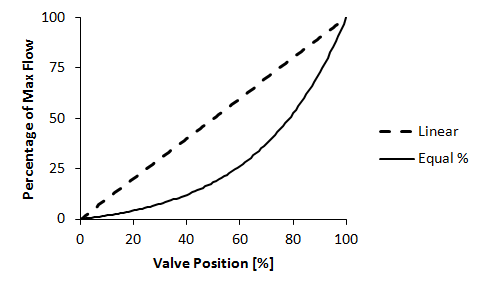
\includegraphics[width=0.55\textwidth]{Graphics/Equal-percentage.png}
	\caption{Valve characteristics}
	\label{fig:equal_percent_valve}
\end{figure}


\subsubsection{Pipe Joining Junction}
Between compressor stage 1, compressor stage 2 and the flash tank (see \cref{fig:HVAC_Diagram}) is a Pipe Joining Junction that connects the three forementioned components.

In \cref{eq:PipeJoiningJunction_ChangeOfMass}, the change of mass inside the Pipe Joining Junction can be expressed as a function of the mass flows into and out of the Pipe Joining Junction.


\begin{equation}
	\tcbhighmath[boxrule = 0.5pt]{ \frac{dM}{dt} = \dot{m}_{in1} + \dot{m}_{in2} - \dot{m}_{out} }       \label{eq:PipeJoiningJunction_ChangeOfMass}   
\end{equation}

where

\begin{center}
	\begin{tabular}{l p{8cm} l}
		$\dfrac{dM}{dt}$ & Change in mass inside Pipe Joining Junction             & [\si{kg}/\si{s}] \\
		$\dot{m}_{in1}$  & Flow into Pipe Joining Junction from Compressor $ C_1 $ & [\si{kg}/\si{s}] \\
		$\dot{m}_{in2}$  & Flow into Pipe Joining Junction from Flash Tank         & [\si{kg}/\si{s}] \\
		$\dot{m_{out}}$  & Flow into Compressor $ C_2 $ from Pipe Joining Junction & [\si{kg}/\si{s}]
	\end{tabular}
\end{center}

In \cref{eq:PipeJoiningJunction_Enthalpy} the specific enthalpy of the flow out of the Pipe Joining Junction is expressed as a function of the input flows and enthalpies. This equation is based on the energy balance, assuming no heat transfer to surroundings, i.e. the Pipe Joining Junction is perfectly insulated. Additionally, it is expected that $\frac{dM}{dt}$ is zero, such that the output mass flow is equal to the sum of the input flows.

\begin{equation} \label{eq:PipeJoiningJunction_Enthalpy}
	h_{out} = \frac{h_{in1} \cdot \dot{m}_{in1} + h_{in2} \cdot \dot{m}_{in2}}{ \dot{m}_{in1} + \dot{m}_{in2} }
\end{equation}

where

\begin{center}
	\begin{tabular}{l p{10cm} l}
		$h_{out}$       & Specific enthalpy into Compressor $ C_2 $ from Pipe Joining Junction & [\si{J}/\si{kg}] \\
		$h_{in1}$       & Specific enthalpy into Pipe Joining Junction from Compressor $ C_1 $ & [\si{J}/\si{kg}] \\
		$h_{in2}$       & Specific enthalpy into Pipe Joining Junction from Flash Tank         & [\si{J}/\si{kg}] \\
		$\dot{m}_{in1}$ & Flow into Pipe Joining Junction from Compressor $ C_1 $              & [\si{kg}/\si{s}] \\
		$\dot{m}_{in2}$ & Flow into Pipe Joining Junction from Flash Tank                      & [\si{kg}/\si{s}]
	\end{tabular}
\end{center}


%\subsubsection{Pipe Splitting Junction}

%This component is particularly simple, as the only function of it is to split the input flow in two. It is furthermore assumed that the dynamics are fast enough that the they can be modelled as algebraic equations.
%
%\begin{equation} \label{eq:PipeSplittingJunction_Enthalpy}
%	\begin{split}
%		\dot{m}_{in} &= \dot{m}_{out1} + \dot{m}_{out2} \\
%		p_{out1} &= p_{in} \\
%		p_{out2} &= p_{in} \\
%		h_{out1} &= h_{in} \\
%		h_{out1} &= h_{in} \\
%	\end{split}
%\end{equation}
%
%where
%
%\begin{center}
%	\begin{tabular}{l p{12cm} l}
%		$\dot{m}_{in}$ 		& Mass flow into Pipe Splitting Junction from Condenser (reciever?) 						& [\si{kg}/\si{s}]\\
%		$\dot{m}_{out1}$ 	& Mass flow into Economiser expansion valve from Pipe Splitting Junction 				& [\si{kg}/\si{s}]\\
%		$\dot{m}_{out2}$ 	& Mass flow into Economiser heat exchanger from Pipe Splitting Junction 					& [\si{kg}/\si{s}]\\
%		$p_{in}$ 			& Absolute pressure input Pipe Splitting Junction from Condenser (reciever?)		& [\si{Pa}]\\
%		$p_{out1}$ 			& Absolute pressure into Economiser expansion valve from Pipe Splitting Junction 	& [\si{Pa}]\\
%		$p_{out2}$ 			& Absolute pressure into Economiser heat exchanger from Pipe Splitting Junction 	& [\si{Pa}]\\
%		$h_{in}$ 			& Specific enthalpy into Pipe Splitting Junction from Condenser (reciever?)   		& [\si{J}/\si{kg}]\\
%		$h_{out1}$ 			& Specific enthalpy into Economiser expansion valve from Pipe Splitting Junction	& [\si{J}/\si{kg}]\\
%		$h_{out2}$ 			& Specific enthalpy into Economiser heat exchanger from Pipe Splitting Junction		& [\si{J}/\si{kg}]\\
%	\end{tabular}
%\end{center}
%
%
%The pressure and specific enthalpy on the output flows are equal to the input pressure and specific enthalpy. The sum of the mass flows out of the Pipe Splitting Junction is equal to the input mass flow. \\

\subsubsection{Compressor}
The compressor in the refrigeration cycle consists of two compressor stages that can be described by the same equations. The compressor type is a scroll compressor.
The compressor dynamics are assumed to be fast enough compared with the refridgeration cycle that it can be considered constant. Therefore, the equations governing the compressors are algebraic equations.
Adiabatic compression is assumed.
The two equations describing the compression governs the mass flow in \cref{eq:comp_mass_flow} and the output specific enthalpy in \cref{eq:comp_enthalpy}. The output specific enthalpy is found via a lookup table $ \Upsilon $ also known as HTP.

\begin{align}
	\dot{m} &= \left(\frac{V_1}{v_1} - \frac{V_C}{v_2}\right) \frac{\omega}{2} \label{eq:comp_mass_flow} \\
	h_{out} &= \Upsilon(T_{out}, p_{out}) \label{eq:comp_enthalpy}
\end{align}

where

\begin{center}
	\begin{tabular}{l p{8cm} l}
		$\dot{m}$  & Flow through compressor stage                                   & [\si{kg}/\si{s}]     \\
		$h_{out}$  & Compressor stage output specific enthalpy                       & [\si{J}/\si{kg}]     \\
		$V_1$      & Cylinder internal volume b.f. 'stroke'                          & [$\si{m}^3$]         \\
		$V_C$      & Cylinder clearance volume after 'stroke'                        & [$\si{m}^3$]         \\
		$v_1$      & Refrigerant specific volume b.f. 'stroke'                       & [$\si{m}^3/\si{kg}$] \\
		$v_2$      & Refrigerant specific volume after 'stroke'                      & [$\si{m}^3/\si{kg}$] \\
		$\omega$   & Compressor angular velocity                                     & [\si{rad}/\si{s}]    \\
		$\Upsilon(T,p)$ & HTP; Lookup table of the enthalpy from temperature and pressure & [$\cdot]$            \\
		$T_{out}$  & Compressor stage output temperature                             & [\si{K}]             \\
		$p_{out}$  & Compressor stage output pressure                                & [\si{Pa}]
	\end{tabular}
\end{center}

In \cref{eq:comp_mass_flow} $v_1$ is found from table lookup as in \cref{eq:comp_prestroke_spec_vol}.

\begin{align}
	v_1 &= \Gamma(T_{in},p_{1}) \label{eq:comp_prestroke_spec_vol} \\
	v_2 &= \left(\frac{p_2}{p_1}\right)^{\frac{-1}{\gamma}} \\
	p_1 &= p_{in} - kl_1 \cdot \omega \\
	p_2 &= p_{out} + kl_2 \cdot \omega \\
	\gamma &= C_{cp}/C_{cv} \\
	T_{in} &= \Phi(h_{in}, p_{in})  \\
	T_{out} &= T_{in}\cdot \left(\frac{p_{out}}{p_{in}}\right)^{\frac{\gamma-1}{\gamma}}
\end{align}

where

\begin{center}
	\begin{tabular}{l p{8cm} l}
		$\Gamma(T,p)$   & VTP; Lookup table of the specific volume from temperature and pressure & [\si{Pa}]                         \\
		$p_{in}$        & Compressor stage input pressure                                        & [\si{Pa}]                         \\
		$p_1$           & 'Piston' input pressure                                                  & [\si{Pa}]                         \\
		$p_2$           & 'Piston' output (discharge) pressure                                     & [\si{Pa}]                         \\
		$\gamma$        & Heat capacity ratio                                                    & [$ \cdot $]                       \\
		$ kl_1$, $kl_2$ & Valve loss constants                                                   & [$ \cdot $]                       \\
		$\omega$        & Compressor angular velocity                                            & [\si{rad}/\si{s}]                 \\
		$T_{in}$        & Compressor stage input temperature                                     & [\si{K}]                          \\
		$C_{cp}$        & Specific heat capacity - constant pressure                             & [\si{J}/(\si{kg}$ \cdot $\si{K})] \\
		$C_{cv} $       & Specific heat capacity - constant volume                               & [\si{J}/(\si{kg}$ \cdot $\si{K})] \\
		$\Phi(h,p)$ 	& TPH; Table lookup of the vapor refrigerant temperature from pressure and enthalpy & [\si{K}]
	\end{tabular}
\end{center}


%\subsubsection{Fan}
%The fans used to move air over the condenser and evaporator are driven by VFD allowing for an assumed continous range of speed settings from 0\% to 100\%. The mass flow as a function of fan speed can be modelled with a 2nd order polynomial, as shown below.
%
%The airflows over the evaporator and condenser are dynamic in themselves, as the airflow is driven by fans that have rotational inertia. Additionally, as the air is a fluid by itself, it contains some inetia too. This behaviour is modeled by:
%
%\begin{align}
%	U_* & = (U_{fan} - 2270.4)\cdot 0.0017 \\
%	\bar{\dot{V}}_{air} & = 0.7273 + 0.1202 \cdot U_*  -0.0044 \cdot U_*^2\\
%	\bar{\dot{m}}_{air} & = \bar{\dot{V}}_{air} \cdot \rho_{air}  \label{eq:Evaporator_FanAirInstantMassFlow}\\
%	%	\bar{\dot{m}}_{air} & = \frac{U_{fan}^2 \cdot 3400.5 + U_{fan}^3 \cdot -1103.5} {3600 \cdot \rho_{air}} \label{eq:Evaporator_FanAirInstantMassFlow}\\
%	\frac{\Delta \dot{m}_{air}}{\Delta t} & = \frac{\bar{\dot{m}}_{air}  - \dot{m}_{air}} {10s} \label{eq:Evaporator_FanAirRateOfChange}
%\end{align}
%
%where
%
%\begin{center}
%	\begin{tabular}{l p{8cm} l}
%		$ U_* $ 								& Intermediate variable												& [1/\si{s}]\\
%		$\bar{\dot{V}}_{air}$						& Estimated steady state volume flow of air for a given fan speed 	& [\si{m^3}/\si{s}] \\
%		$\bar{\dot{m}}_{air}$						& Estimated steady state mass flow of air for a given fan speed 	& [\si{kg}/\si{s}] \\
%		$\dot{m}_{air}$								& Actual mass flow of air					  						& [\si{kg}/\si{s}] \\
%		$U_{fan}$									& Fan speed 														& [1/\si{s}] \\
%		$\rho_{air}$								& Density of air													& [\si{kg}/\si{m^3}] \\[0.2cm]
%		$\dfrac{\Delta \dot{m}_{air}}{\Delta t} $ 	& The rate of change of	air flow 									& [\si{kg}/\si{s^2}]
%	\end{tabular}
%\end{center}
%
%\cref{eq:Evaporator_FanAirInstantMassFlow} calculates the steady state air mass flow at new speed. \cref{eq:Evaporator_FanAirRateOfChange} approximates the rate of change of the air mass flow as a first-order difference with time constant of 10 seconds. \\



\subsubsection{Condenser}

The condenser takes in the discharge pressure vapor from the second compressor stage, at point 4 in \cref{fig:HVAC_Diagram}. The high pressure yields a high temperature,
which enables heat transfer through the condensor to ambient air. This is done mainly through condensation of the refrigerant vapor, yielding high pressure liquid at point 5 in \cref{fig:HVAC_Diagram}.
The energy balance is modelled in \cref{eq:Condenser_Enthalpy}. The mass balance is modelled in \cref{eq:Condenser_ChangeOfMass}. Finally the temperature of the metal in the condenser is modelled in
\cref{eq:Condenser_ChangeOfTemperature}, as the dominant dynamics of the condenser is greatly linked to the temperature of the metal \cite{Sorensen2013}. \cref{eq:Condenser_ChangeOfTemperature} is also
derived from the energy balance. In \cref{fig:condenser_CV} a diagram of the condenser CV can be found.

\begin{figure}[h!]
	\centering
	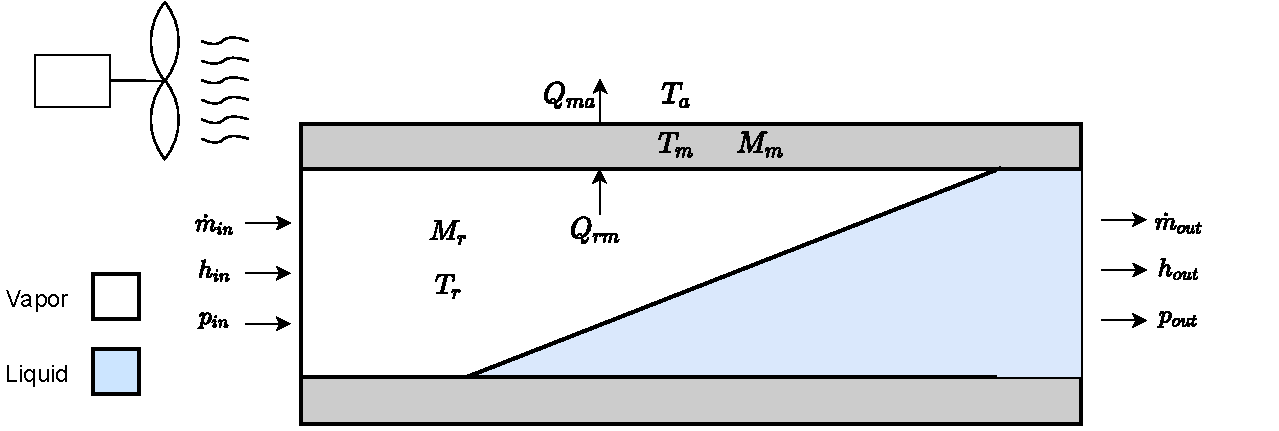
\includegraphics[width=0.8\textwidth]{Graphics/Condenser.pdf}
	\caption{Diagram of condenser control volume}
	\label{fig:condenser_CV}
\end{figure}

\begin{align}
	h_{out} 			& = h_{in} - \frac{Q_{rm}}{\dot{m}_{in}}  	\label{eq:Condenser_Enthalpy} \\
\end{align}

\begin{equation}
	\tcbhighmath[boxrule = 0.5pt]{ 	\frac{dM_r}{dt} 	 = \dot{m}_{in}(t) - \dot{m}_{out}(t) }     	\label{eq:Condenser_ChangeOfMass}   
\end{equation}
\begin{equation}
	\tcbhighmath[boxrule = 0.5pt]{ 	\frac{dT_m}{dt} 	 = \frac{Q_{rm} - Q_{ma}}{M_m \cdot Cp_m}	 }     \label{eq:Condenser_ChangeOfTemperature}      
\end{equation}



where

\begin{center}
	\begin{tabular}{l p{8cm} l}
		$h_{out}$       & Condenser output specific enthalpy & [\si{J}/\si{kg} ] \\
		$h_{in}$        & Condenser input specific enthalpy  & [\si{J}/\si{kg}]  \\
		$Q_{rm}$        & Refrigerant to metal heat flow     & [\si{W}]          \\
		$Q_{ma}$        & Metal to air heat flow             & [\si{W}]          \\
		$\dot{m_{in}}$  & Condenser input mass flow          & [\si{kg}/\si{s}]  \\
		$\dot{m_{out}}$ & Condenser output mass flow         & [\si{kg}/\si{s}]  \\
		$M_r$           & Refrigerant mass                   & [\si{kg}]         \\
		$M_m$           & Metal mass                         & [\si{kg}]         \\
		$T_m$           & Metal temperature                  & [\si{K}]          \\
		$Cp_m$          & Metal heat capacity                & [\si{J}/\si{K}]
	\end{tabular}
\end{center}

The pressure drop across the condenser is assumed to be linear with respect to mass flow, yielding \cref{eq:Condenser_PressureDrop}.
The mass flow out of the condenser is modelled in \cref{eq:Condenser_MassFlow}.


\begin{align}
	p_{in} 	& =  p_{out} - \lambda \cdot \dot{m}_{in}  				\label{eq:Condenser_PressureDrop}\\
	\dot{m}_{out}		& = \dot{m}_{in} + \frac{M_r - \frac{V_i}{v}}{1s}		\label{eq:Condenser_MassFlow} \\
	v & = \mathcal{Z}(h_{in}, p_{in})
\end{align}

where

\begin{center}
	\begin{tabular}{l p{8cm} l}
		$p_{in}$        & Condenser input pressure                                   & [\si{Pa}]          \\
		$p_{out}$       & Condenser output pressure                                  & [\si{Pa}]          \\
		$\lambda$       & Pressure drop constant                                     & [$\cdot$]          \\
		$\dot{m_{in}}$  & Condenser input mass flow                                  & [\si{kg}/\si{s}]   \\
		$\dot{m_{out}}$ & Condenser output mass flow                                 & [\si{kg}/\si{s}]   \\
		$M_{r}$         & Condenser refridgerant mass                                & [\si{kg}]          \\
		$V_{i}$         & Condenser internal volume                                  & [\si{m^3}]         \\
		$v$             & Condenser refridgerant specific volume                     & [\si{m^3}/\si{kg}] \\
		$\mathcal{Z}(h,p)$        & Table lookup of specific volume from enthalpy and pressure & []
	\end{tabular}
\end{center}


And finally the convective heat flows are modelled in \cref{eq:Condenser_HeatFlow_rm}, \cref{eq:Condenser_HeatFlow_ma}. The heat flow from metal to air is assumed to be approximately proportional to the air flow, which is why the speed of the fan is multiplied to the energy flow in \cref{eq:Condenser_HeatFlow_ma}. There is an offset of 0.05 times the energy flow to account for the fact that there will exist a heat flow when the fan is not operating.

\begin{align}
	Q_{rm}	 			& = U A_{rm} \cdot (T_r - T_m)							\label{eq:Condenser_HeatFlow_rm}\\
	Q_{ma}	 			& = U A_{ma} \cdot (T_m - T_{ambi})\cdot (0.05 + U_{fan} \cdot 2)				\label{eq:Condenser_HeatFlow_ma}
\end{align}

where

\begin{center}
	\begin{tabular}{l p{8cm} l}
		$Q_{rm}$				&	Heat flow from refridgerant to metal					& [\si{W}] \\
		$Q_{ma}$				&	Heat flow from metal to air								& [\si{W}] \\
		$U A_{rm}$				& 	Heat transfer coefficient from refridgerant to metal 	& [\si{J}/\si{K}] \\
		$U A_{ma}$				& 	Heat transfer coefficient from metal to air				& [\si{J}/\si{K}] \\
		$T_r$					& 	Temperature of refridgerant 							& [\si{K}] \\
		$T_m$					&	Temperature of metal 									& [\si{K}] \\
		$T_{ambi}$				&	Temperature of ambient air 								& [\si{K}] \\
		$U_{fan}$				&	Fan speed												& [$\%$] \\
	\end{tabular}
\end{center}

All the equations until now has been heavily inspired by \cite{Sorensen2013}.
Now, to accommodate the missing pressure $ p_{out} $ from \cref{eq:Condenser_PressureDrop}, an new state is needed for the pressure in the condenser which will be assumed to be the output pressure. The following shows the derivation of that state from the mass balance in \cref{eq:Condenser_ChangeOfMass}. We use the fact that the mass in the control volume consists of two seperate masses, the liquid mass $ M_l $ and the vapor mass $ M_v $.


\begin{align}
		 		\frac{d \bigl(M_{l} + M_{v}\bigr) }{dt} & = \dot{m}_{in}(t) - \dot{m}_{out}(t) 		\label{eq:Condenser_pres1}\\
		 		\frac{d \Bigl(\rho_{l}\bigl(p(t)\bigr)\cdot V_l(t) + \rho_{v}\bigl(p(t)\bigr)\cdot \bigl(V_{tot} - V_l(t)\bigr)\Bigr) }{dt} & = \dot{m}_{in}(t) - \dot{m}_{out}(t)		\label{eq:Condenser_pres2}\\
		 		\frac{d \Bigl(\rho_{l}\bigl(p(t)\bigr)\cdot V_l(t)\Bigr)}{dt} + \frac{d \Bigl(\rho_{v}\bigl(p(t)\bigr)\cdot \bigl(V_{tot} - V_l(t)\bigr)\Bigr) }{dt} & = \dot{m}_{in}(t) - \dot{m}_{out}(t)		\label{eq:Condenser_pres3}
\end{align}

where $\rho_{l}, \rho_{v}$ are the densities of respectively are the densities of saturated liquid and saturated vapor. $ V_l$ is the volume of the liquid part of the control volume, $V_{tot} $ is the total volume of the control volume, which is the volume of the condenser and $p(t)$ is the pressure inside the control volume. 

Utilizing the product rule for differentiation for each of the derivative terms on the LHS of \cref{eq:Condenser_pres3} yields \cref{eq:Condenser_pres4} and \cref{eq:Condenser_pres5}.
\begin{align}
	\frac{d \Bigl(\rho_{l}\bigl(p(t)\bigr)\cdot V_l(t)\Bigr)}{dt}  				& =   \frac{d \rho_{l}\bigl(p(t)\bigr)}{dt} \cdot V_l(t)   +   \rho_{l}\bigl(p(t)\bigr)\cdot\frac{d V_l(t)}{dt} 	\label{eq:Condenser_pres4} \\
	\frac{d \Bigl(\rho_{v}\bigl(p(t)\bigr)\cdot (V_{tot} - V_l(t))\Bigr) }{dt} 	& =  \frac{d \rho_{v}\bigl(p(t)\bigr)}{dt} \cdot \bigl(V_{tot} - V_l(t)\bigr)   +   \rho_{v}\bigl(p(t)\bigr)\cdot\frac{d \bigl(V_{tot} - V_l(t)\bigr)}{dt} 	\label{eq:Condenser_pres5}
\end{align}
The first term of the RHS of \cref{eq:Condenser_pres4} and \cref{eq:Condenser_pres5} can then be expanded using the chain rule as seen in \cref{eq:Condenser_pres6}

\begin{align}
	\frac{d \rho_{l}\bigl(p(t)\bigr)}{dt} 				& =   \frac{d \rho_{l}\bigl(p(t)\bigr)}{dp(t)} \cdot \frac{dp(t)}{dt}	\label{eq:Condenser_pres6} \\
		\frac{d \rho_{v}\bigl(p(t)\bigr)}{dt} 			& =   \frac{d \rho_{v}\bigl(p(t)\bigr)}{dp(t)} \cdot \frac{dp(t)}{dt}	\label{eq:Condenser_pres7}
\end{align}

Now the RHS of \cref{eq:Condenser_pres4} and \cref{eq:Condenser_pres5} are substituted into the LHS of \cref{eq:Condenser_pres3} yielding \cref{eq:Condenser_pres8}. \\

%\begin{align}
%			 		\frac{d \rho_{l}\bigl(p(t)\bigr)}{dt} \cdot V_l(t)   +   \rho_{l}\bigl(p(t)\bigr)\cdot\frac{d V_l(t)}{dt} +
%			 		\frac{d \rho_{v}\bigl(p(t)\bigr)}{dt} \cdot (V_{tot} - V_l(t))   +   \rho_{v}\bigl(p(t)\bigr)\cdot\frac{d (V_{tot} - V_l(t))}{dt}
%			 			& = \dot{m}_{in}(t) - \dot{m}_{out}(t)  \label{eq:Condenser_pres8}
%\end{align}

\begin{equation}\label{eq:Condenser_pres8}
	\begin{split}
		& \frac{d \rho_{l}\bigl(p(t)\bigr)}{dt} \cdot V_l(t)   +   \rho_{l}\bigl(p(t)\bigr)\cdot\frac{d V_l(t)}{dt} +
		\frac{d \rho_{v}\bigl(p(t)\bigr)}{dt} \cdot \bigl(V_{tot} - V_l(t)\bigr)   +   \rho_{v}\bigl(p(t)\bigr)\cdot\frac{d \bigl(V_{tot} - V_l(t)\bigr)}{dt} \\
		& = \dot{m}_{in}(t) - \dot{m}_{out}(t)
	\end{split}
\end{equation}


\cref{eq:Condenser_pres6} and \cref{eq:Condenser_pres7} are substituted into \cref{eq:Condenser_pres8} yielding \cref{eq:Condenser_pres9}.

\begin{equation}\label{eq:Condenser_pres9}
	\begin{split}
		& \frac{d \rho_{l}\bigl(p(t)\bigr)}{dp(t)} \cdot \frac{dp(t)}{dt} \cdot V_l(t)   +   \rho_{l}\bigl(p(t)\bigr)\cdot\frac{d V_l(t)}{dt} +  \frac{d \rho_{v}\bigl(p(t)\bigr)}{dp(t)} \cdot \frac{dp(t)}{dt} \cdot \bigl(V_{tot} - V_l(t)\bigr)   +
		\rho_{v}\bigl(p(t)\bigr)\cdot\frac{d \bigl(V_{tot} - V_l(t)\bigr)}{dt}  \\ &= \dot{m}_{in}(t) - \dot{m}_{out}(t)
	\end{split}
\end{equation}

To simplify the equation we assume that the volumes of the liquid and vapor parts are constant, i.e. $ V_l(t) = V_l$, yielding \cref{eq:Condenser_pres10}, where the derivatives if the volumes are neglected.

\begin{align}
		\frac{d \rho_{l}\bigl(p(t)\bigr)}{dp(t)} \cdot \frac{dp(t)}{dt} \cdot V_l +  \frac{d \rho_{v}\bigl(p(t)\bigr)}{dp(t)} \cdot \frac{dp(t)}{dt} \cdot \bigl(V_{tot} - V_l\bigr) & = \dot{m}_{in}(t) - \dot{m}_{out}(t) \label{eq:Condenser_pres10} \\
		 \frac{dp(t)}{dt} \cdot \Biggl( \frac{d \rho_{l}\bigl(p(t)\bigr)}{dp(t)} \cdot V_l +  \frac{d \rho_{v}\bigl(p(t)\bigr)}{dp(t)} \cdot \bigl(V_{tot} - V_l\bigr) \Biggr) & = \dot{m}_{in}(t) - \dot{m}_{out}(t) \label{eq:Condenser_pres11}
\end{align}
Now the state equation for the pressure can be found by isolating $ \frac{p(t)}{dt} $ as in \cref{eq:Condenser_pres12}
\begin{align}
	\frac{dp(t)}{dt} & = \dfrac{\dot{m}_{in}(t) - \dot{m}_{out}(t)}{ \dfrac{d \rho_{l}\bigl(p(t)\bigr)}{dp(t)} \cdot V_l +  \dfrac{d \rho_{v}\bigl(p(t)\bigr)}{dp(t)} \cdot \bigl(V_{tot} - V_l\bigr) } \label{eq:Condenser_pres12}
\end{align}

Table lookups can be used to evaluate the derivatives of the density with respect to the pressure. This will be signified by the notation in \cref{eq:Condenser_pres13} for respectively saturated vapor and saturated liquid.

\begin{align}
		\dfrac{d \rho_l\bigl(p(t)\bigr)}{dp(t)} = \left. \dfrac{d \rho_l\bigl(p\bigr)}{dp} \right |_{p = p(t)} & = \mathcal{F}(p(t)) \label{eq:Condenser_pres13} \\
		\dfrac{d \rho_v\bigl(p(t)\bigr)}{dp(t)} = \left. \dfrac{d \rho_v\bigl(p\bigr)}{dp} \right |_{p = p(t)} & = \mathcal{G}(p(t)) \label{eq:Condenser_pres14}
\end{align}

Finally we arrive at the state equation \cref{eq:Condenser_pres15} for the pressure state in the condenser control volume.

\begin{equation} 
	\tcbhighmath[boxrule = 0.5pt]{\frac{dp(t)}{dt} = \dfrac{\dot{m}_{in}(t) - \dot{m}_{out}(t)}{ \mathcal{F}(p(t)) \cdot V_l +  \mathcal{G}(p(t))) \cdot \bigl(V_{tot} - V_l\bigr) }}\label{eq:Condenser_pres15}
\end{equation}

We can now proceed to the next component for the reefer trailer model.

\subsubsection{Flash tank}
The flash tank in combination with the condenser throttle valve serves to reduce the amount of high enthalpy flash gas delivered to the evaporator. The condenser throttle valve, whose model is identical to the expansion valve, lowers the pressure of the liquid from the condenser. This naturally lowers the temperature, but also generates some amount of flash gas. The flash tank then separates the liquid-vapor mixture and passes only the liquid to the expansion valve. The flash gas is returned to the second stage of the compressor, where it is reused. Thus, a lower amount of flash gas will be generated by the expansion valve, as the pressure of the liquid is already lowered, and the resulting flash gas from the condenser throttle valve is led to compressor stage 2.

The modeling will only evaluate the steady state behaviour of the flash tank due to the limited scope of the project. A diagram of the flash tank can be seen in \cref{fig:flash_tank_CV}

\begin{figure}[h!]
	\centering
	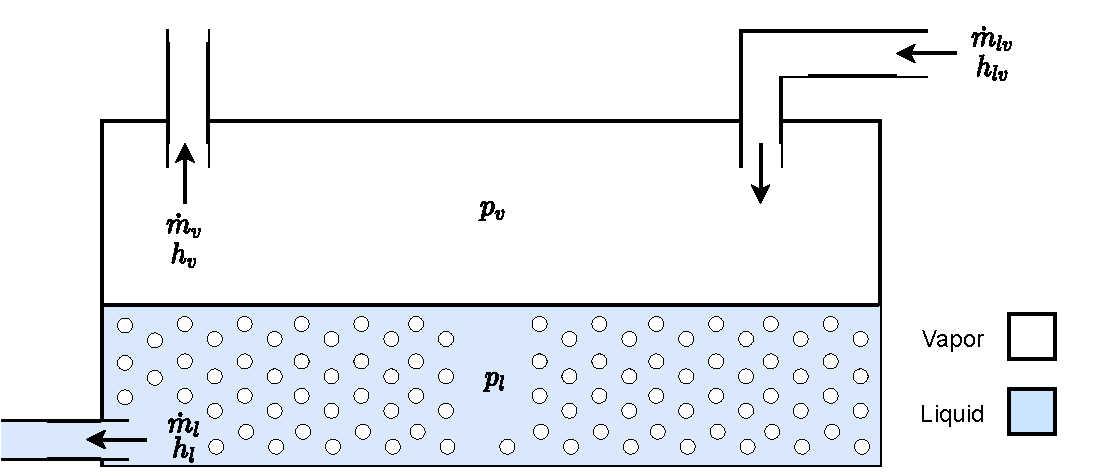
\includegraphics[width=0.65\textwidth]{Graphics/Flash_tank.pdf}
	\caption{Diagram of Flash tank control volumes}
	\label{fig:flash_tank_CV}
\end{figure}

In steady state it is firstly assumed that the pressure of the liquid-vapor mixture entering is the same as the separated liquid and vapor leaving the tank.
\begin{align}
	p_{lv} 	= p_{l}					&  = p_{v}
	\label{eq:Flash_tank_pressure}
\end{align}

where

\begin{center}
	\begin{tabular}{l p{8cm} l}
		$p_{lv}$				&  Liquid-vapor mixture pressure		& [\si{Pa}]\\
		$p_{l}$					&  Liquid pressure 						& [\si{Pa}] \\
		$p_{v}$					&  Vapor pressure						& [\si{Pa}]\\

	\end{tabular}
\end{center}


Secondly, it is assumed that the energy of the mixture and mass of mixture does not change, meaning the energy flow and mass flow in equals the energy flow and mass flow out respectively.

\begin{align}
	\dot{m}_{lv} \cdot  h_{lv}  - \dot{m}_{l} \cdot  h_{l} - \dot{m}_{v} \cdot  h_{v} & = 0 \label{eq:Flash_tank_energyflow} \\
	\dot{m}_{lv} - \dot{m}_{l} - \dot{m}_{v} & = 0  \label{eq:Flash_tank_massflow} \\
\end{align}

where

\begin{center}
	\begin{tabular}{l p{8cm} l}
		$\dot{m}_{lv}$			&  Liquid-vapor mixture mass flow			& [\si{kg}/\si{s}]\\
		$\dot{m}_{l}$			&  Liquid mass flow 						& [\si{kg}/\si{s}] \\
		$\dot{m}_{v}$			&  Vapor mass flow							& [\si{kg}/\si{s}]\\
		$h_{lv}$				&  Liquid-vapor mixture specific enthalpy	& [\si{J}/\si{kg}]\\
		$h_{l}$					&  Liquid specific enthalpy 				& [\si{J}/\si{kg}] \\
		$h_{v}$					&  Vapor specific enthalpy					& [\si{J}/\si{kg}]\\

	\end{tabular}
\end{center}


Lastly, it is assumed that the separated liquid and vapor leaves at boiling point and flash point respectively. This last assumption allows us to find the enthalpy of the two substances purely from investigation of the p-h diagram or a look-up table since the pressure is known. We express this as:

\begin{align}
	h_{l}  & = \mathcal{M}(p)\\
	h_{v}  & = \mathcal{N}(p)
\end{align}

where

\begin{center}
	\begin{tabular}{l p{8cm} l}
		$\mathcal{M}(p)$ & Lookup table of bubble point specific enthalpy from pressure & [\si{J}/\si{kg}] \\
		$\mathcal{N}(p)$ & Lookup table of dew point specific enthalpy from pressure    & [\si{J}/\si{kg}]
	\end{tabular}
\end{center}

The knowledge of the specific enthalpy from the look up tables leaves \cref{eq:Flash_tank_energyflow} and \cref{eq:Flash_tank_massflow} with two unknowns that can be solved, namely $ m_l $ and $ m_v $.

\subsubsection{Subcooling throttle}
The subcooling throttle valve is used differently from the two other valves in the system. During normal operation it is fully open, acting as a pipe. It can be closed fully allowing for various speciel functionalities. Firstly, shutting it off allows for detecting the amount of refridgerant in the system. This is a convenient diagnostic feature which helps ensuring that the system has enough refridgerant to properly function, and enabling leakage detection. Secondly, closing the valve while fully opening the condenser throttle valve, allows the system to operate as a standard refridgeration system, with only one valve between the evaporator and condenser.


\subsubsection{Evaporator}
The superheat of the evaporator is an important and difficult state to control. It is important as the compressor can be damaged if the refrigerant contains liquid. Additionally the superheat is important from an efficiency point of view.
The superheat is the difference between the vapor saturation temperature and the actual temperature at the compressor suction inlet. It is a measure of excess energy transferred to the refrigerant.

% This clearpage might be removed. I just put it here because it was looking ugly at the time.
\clearpage

\begin{figure}[h!]
	\centering
	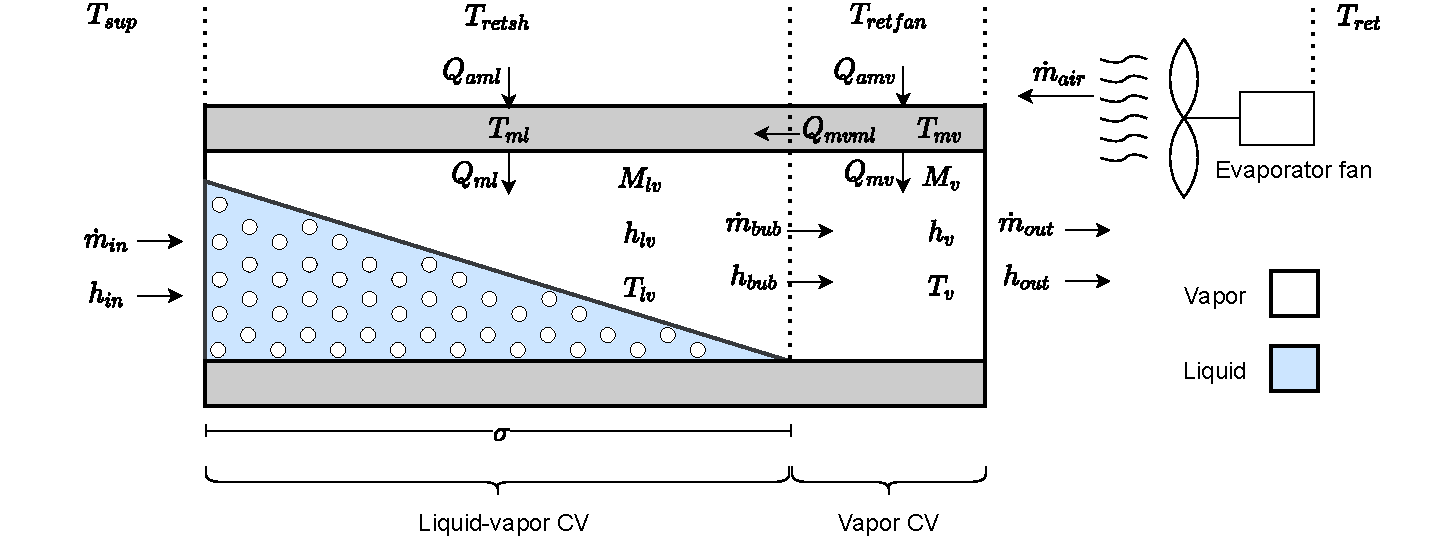
\includegraphics[width=0.8\textwidth]{Graphics/Evaporator_CV_diagram.pdf}
	\caption{Diagram of evaporator control volumes}
	\label{fig:evap_CV}
\end{figure}

The evaporator is split into two control volumes, divided by a moving control volume boundary $\sigma$ which divides liquid-vapor mixture and the superheated vapor, see \cref{fig:evap_CV}.

Because the heat transfer coefficient from liquid to metal and from vapor to metal is different, the metal is likewise split by the $\sigma$ boundary. The modeling of $\sigma$ is based on an assumption that the refrigerant has a constant average quality ($X_e = 0.1$) throughout the liquid-vapor mixture. The specific volume $v_1$ is then found from the output pressure ($p_{out}$) and said average quality constant.

The calculation of the boundary location can be seen in \cref{eq:Evaporator_boundary}.

\begin{align} \label{eq:Evaporator_boundary}
	\sigma = \frac{M_{lv} \cdot v_1}{V_i} \\
	v_1 = \Lambda(p_{out},X_e)
\end{align}

where

\begin{center}
	\begin{tabular}{l p{10cm} l}
		$\sigma$   & Control Volume boundary                                           & [$\cdot$]            \\
		$M_{lv}$   & Mass of liquid-vapor CV                                           & [\si{kg}]            \\
		$v_1$      & Refrigerant specific volume of vapor-liquid CV                    & [$\si{m}^3/\si{kg}$] \\
		$V_i$      & Evaporator volume                                                 & [$\si{m}^3$]         \\
		$\Lambda(p,X)$ & Table lookup of specific volume from pressure and average quality & [$\si{m}^3$]
	\end{tabular}
\end{center}

\medskip
The temperatures of the air which is blown over the evaporator by the fan is modeled by the two equations below. The fan has some loss in the form of heat which is transferred to the air.

\begin{align}
	T_{retfan} 		& = T_{ret} + \frac{Q_{fan}}{\dot{m}_{air} \cdot Cp_{air}} 		\label{eq:T_retfan} 		\\
	T_{retsh} 		& = T_{retfan} - \frac{Q_{amv}}{\dot{m}_{air} \cdot Cp_{air}} 	\label{eq:T_retsh}
\end{align}

where

\begin{center}
	\begin{tabular}{l p{10cm} l}
		$T_{retfan}$    & Temperature of return air after passing through fan & [\si{K}]                          \\
		$T_{retsh}$     & Temperature of air over superheated vapor CV        & [\si{K}]                          \\
		$T_{ret}$       & Return temperature of air coming from trailer       & [\si{K}]                          \\
		$Q_{fan}$       & Heat added from fan to air (heatloss)               & [\si{W}]                          \\
		$Q_{amv}$       & Heat flow from air to metal surrounding vapor CV    & [\si{W}]                          \\
		$\dot{m}_{air}$ & Mass flow of air through fan                        & [\si{kg}/\si{s}]                  \\
		$Cp_{air}$      & Specific heat capacity of air                       & [\si{J}/(\si{K}$ \cdot $\si{kg})]
	\end{tabular}
\end{center}

\medskip
The heat flow from air to metal of evaporator is modeled based on the assumption that the mass flow of air is cooled down to the metal temperature as seen in \cref{eq:Q_amv} and \cref{eq:Q_aml}.

\cref{eq:Q_fan_heatloss} is the heat loss from the fan that is being added to the air flow.

\begin{align}
	U_{*_P} & = \left( U_{fan}\cdot 100 - 55.56 \right) \cdot 0.0335                                         \\
	Q_{fan} & = 177.76 + 223.95 \cdot U_{*_P} + 105.85 \cdot U_{*_P}^2 + 16.74 \cdot U_{*_P}^3	\label{eq:Q_fan_heatloss} \\
	Q_{amv} & = Cp_{air} \cdot \dot{m}_{air} \cdot (T_{retfan} - T_{mv}) 	\label{eq:Q_amv}                                \\
	Q_{amlv} & = Cp_{air} \cdot \dot{m}_{air} \cdot (T_{retsh} - T_{mlv}) 	\label{eq:Q_aml}
\end{align}

where

\begin{center}
	\begin{tabular}{l p{10cm} l}
		$U_{*_P}$       & Transformed fan speed                                & [1/\si{s}]                        \\
		$U_{fan}$       & Fan speed                                            & [$\%$]                        \\
		$Q_{fan}$       & Heat flow from fan to air (heatloss)                 & [\si{W}]                          \\
		$Q_{amv}$       & Heat flow from air to metal surrounding vapor CV     & [\si{W}]                          \\
		$Cp_{air}$      & Specific heat capacity of air                        & [\si{J}/(\si{K}$ \cdot $\si{kg})] \\
		$\dot{m}_{air}$ & Mass flow of air through fan                         & [\si{kg}/\si{s}]                  \\
		$T_{retfan}$    & Temperature of return air after passing through fan  & [\si{K}]                          \\
		$T_{mv}$        & Temperature of metal surrounding the vapor CV        & [\si{K}]                          \\
		$T_{mlv}$       & Temperature of metal surrounding the liquid-vapor CV & [\si{K}]
	\end{tabular}
\end{center}

The fans used to move air over the condenser and evaporator are driven by VFD allowing for a continuous range of speed settings from 0\% to 100\%. The mass flow as a function of fan speed can be modeled with a 2nd order polynomial, as shown in \cref{eq:evap_Vbardot_air}.

The airflow over the evaporator and condenser are dynamic because they are driven by fans that have rotational inertia. Additionally, as the air is a fluid itself, it contains some inertia too. This behavior is modeled by \cref{eq:evap_U_star_mdot} $\rightarrow$ \cref{eq:Evaporator_FanAirRateOfChange}. \cref{eq:Evaporator_FanAirInstantMassFlow} calculates the estimated steady state air mass flow at a new speed. \cref{eq:Evaporator_FanAirRateOfChange} approximates the rate of change of the air mass flow as a first-order difference with time constant of 10 seconds.

\begin{align}
	U_{*_{\dot{m}}} & = (U_{fan}*3060 - 2270.4)\cdot 0.0017 \label{eq:evap_U_star_mdot}\\
	\bar{\dot{V}}_{air} & = 0.7273 + 0.1202 \cdot 	U_{*_{\dot{m}}}  -0.0044 \cdot 	U_{*_{\dot{m}}}^2	\label{eq:evap_Vbardot_air} \\
	\bar{\dot{m}}_{air} & = \bar{\dot{V}}_{air} \cdot \rho_{air}	\label{eq:Evaporator_FanAirInstantMassFlow} \\
	\frac{\Delta \dot{m}_{air}}{\Delta t} & = \frac{\bar{\dot{m}}_{air}  - \dot{m}_{air}} {10s}	\label{eq:Evaporator_FanAirRateOfChange}
\end{align}

where

\begin{center}
	\begin{tabular}{l p{8cm} l}
		$ 	U_{*_{\dot{m}}} $ 						& Transformed fan speed												& [1/\si{s}]\\
		$\bar{\dot{V}}_{air}$						& Estimated steady state volume flow of air for a given fan speed 	& [\si{m^3}/\si{s}] \\
		$\bar{\dot{m}}_{air}$						& Estimated steady state mass flow of air for a given fan speed 	& [\si{kg}/\si{s}] \\
		$\dot{m}_{air}$								& Actual mass flow of air					  						& [\si{kg}/\si{s}] \\
		$U_{fan}$									& Fan speed 														& [$\%$] \\
		$\rho_{air}$								& Density of air													& [\si{kg}/\si{m^3}] \\[0.2cm]
		$\dfrac{\Delta \dot{m}_{air}}{\Delta t} $ 	& The rate of change of	air flow 									& [\si{kg}/\si{s^2}]
	\end{tabular}
\end{center}

The evaporator contains one of the greater thermal masses due to the large mass of metal in the heat exchanger.The temperature of the evaporator metal is divided into two parts corresponding to the liquid-vapor control volume \cref{eq:evap_dT_ml} and the vapor control volume \cref{eq:evap_dT_mv}. The metal temperature change is governed by the heat flows to and from the metal ($ Q_{amlv}, Q_{mlv}, Q_{mvmlv} $ in \cref{eq:evap_dT_ml} and $ Q_{amv}, Q_{mv}, Q_{mvmlv} $ in \cref{eq:evap_dT_mv}) and the mass of the metal in that CV ($M_m \cdot \sigma$ in \cref{eq:evap_dT_ml} and $M_m \cdot (1 - \sigma)$ in \cref{eq:evap_dT_mv}) multiplied with the specific heat capacity of the metal ($Cp_m$). The heat flows are illustrated in \cref{fig:evap_CV}


\begin{equation}
	\tcbhighmath[boxrule = 0.5pt]{ 	\frac{dT_{mlv}}{dt}  = \frac{Q_{amlv}-Q_{mlv} + Q_{mvmlv}}{M_m \cdot \sigma \cdot Cp_m}  }    \label{eq:evap_dT_ml}        
\end{equation}
\begin{equation}
	\tcbhighmath[boxrule = 0.5pt]{ \frac{dT_{mv}}{dt} = \frac{Q_{amv} - Q_{mv} - Q_{mvmlv}}{M_m \cdot (1 - \sigma) \cdot Cp_m } }     \label{eq:evap_dT_mv}       
\end{equation}



where

\begin{center}
	\begin{tabular}{l p{10cm} l}
		$T_{mlv} $  & Metal temperature in liquid-vapor CV                                                        & [\si{K}/\si{s}]                   \\ %[0.3cm]
		$T_{mv} $   & Metal temperature in vapor CV                                                               & [\si{K}/\si{s}]                   \\ %[0.3cm]
		$Q_{amlv}$  & Heat flow from air to metal surrounding liquid-vapor CV                                     & [\si{W}]                          \\
		$Q_{mlv}$   & Heat flow from evaporator metal to liquid-vapor CV                                          & [\si{W}]                          \\
		$Q_{mvmlv}$ & Heat flow from through from metal surrounding vapor CV to metal surrounding liquid-vapor CV & [\si{W}]                          \\
		$Q_{amv}$   & Heat flow from air to metal surrounding vapor CV                                            & [\si{W}]                          \\
		$Q_{mv}$    & Heat flow from evaporator metal to vapor CV                                                 & [\si{W}]                          \\
		$M_{m} $    & Mass of metal                                                                               & [\si{kg}]                         \\
		$Cp_{m}$    & Specific heat capacity of metal                                                             & [\si{J}/(\si{K}$ \cdot $\si{kg})] \\
		$\sigma$    & Control Volume boundary                                                                     & [$\cdot$]
	\end{tabular}
\end{center}

\medskip
\cref{eq:Q_mvml} $\rightarrow$ \cref{eq:Q_mv} model convection heat flows between the metal CVs and to the vapor-liquid and vapor CVs. They are modeled as the temperature difference between two CVs multiplied with the specific heat coefficient between the two. The specific heat coefficients ($U A_1 \rightarrow U A_3$) are found empirically from steady-state tests in \cite{Sorensen2013} for a similar refrigeration system. The temperature of the vapor refrigerant leaving the evaporator is found from output pressure and enthalpy in \cref{eq:T_v}

\begin{align}
	Q_{mvmlv} & = U A_3 \cdot (T_{mv} - T_{mlv}) \label{eq:Q_mvml}             &  \\
	Q_{mlv}   & = U A_1 \cdot (T_{mlv} - T_{lv}) \cdot \sigma	\label{eq:Q_ml}&  \\
	Q_{mv}    & = U A_2 \cdot (T_{mv} - T_v) \cdot (1- \sigma) \label{eq:Q_mv} &  \\
	T_{lv}    & = \Phi(p_{in}, h_{in}) \label{eq:T_v}                          &
\end{align}

where

\begin{center}
	\begin{tabular}{l p{10cm} l}
		$Q_{amlv}$  & Heat flow from air to metal surrounding liquid-vapor CV                           & [\si{W}]        \\
		$Q_{mvmlv}$ & Heat flow from through from vapor CV metal to liquid-vapor CV metal               & [\si{W}]        \\
		$Q_{mlv}$   & Heat flow from evaporator metal to liquid-vapor CV                                & [\si{W}]        \\
		$Q_{mv}$    & Heat flow from evaporator metal to vapor CV                                       & [\si{W}]        \\
		$T_{mlv}$   & Temperature of metal on the liquid-vapor CV                                       & [\si{K}]        \\
		$T_{mv}$    & Temperature of metal on the vapor CV                                              & [\si{K}]        \\
		$T_{lv}$    & Saturation temperature for evaporation of the refrigerant                         & [\si{K}]        \\
		$T_{v}$     & Temperature of refrigerant (vapor) leaving the evaporator                         & [\si{K}]        \\
		$UA_1$      & Heat transfer coefficient from metal to liquid                                    & [\si{J}/\si{K}] \\
		$UA_2$      & Heat transfer coefficient from metal to vapor                                     & [\si{J}/\si{K}] \\
		$UA_3$      & Heat transfer coefficient from vapor CV metal to liquid-vapor CV metal            & [\si{J}/\si{K}] \\
		$\Phi(p,h)$ 		& TPH; Table lookup of the vapor refrigerant temperature from pressure and enthalpy & [\si{K}]
	\end{tabular}
\end{center}

\medskip
The output pressure, specific enthalpies and mass balances are given by equations \cref{eq:evap_pout} $\rightarrow$ \cref{eq:evap_dMvdt}. \cref{eq:evap_Tsup} describes the temperature of the air leaving the evaporator and \cref{eq:evap_mdot_{lv}} describes the flow from the liquid-vapor CV to the vapor CV. The dew point specific enthalpy is the specific enthalpy level in the evaporator where liquid vapor mixture has completely changed phase to vapor. The pressure in \cref{eq:evap_pout} is found from table lookup using the specific volume of the refrigerant in the vapor CV and the specific enthalpy.

\begin{align}
	p_{out}            & = \Pi \left( h_v, \frac{M_v}{V_i-V_{lv}} \right)		\label{eq:evap_pout}                       \\
	V_{lv}             & = \sigma \cdot V_i                                                                           \\
	h_{lv}             & = h_{in} + \frac{Q_{mlv}}{\dot{m}_{in}}                                                      \\
	h_v                & = h_{dew} + \frac{Q_{mv}}{\dot{m}_{dew}}               \label{eq:evap_hv}                                       \\
	h_{out}            & = h_v                                                                                       \\
	T_{out}            & = T_v                                                                                        \\
	T_{sup}            & = T_{retfan} +  \frac{Q_{amlv} + Q_{amv}}{Cp_{air} \cdot \dot{m}_{air}} \label{eq:evap_Tsup} \\
	\dot{m}_{dew}      & = \frac{Q_{mlv}}{h_{dew} - h_{in}} \label{eq:evap_mdot_{lv}}
\end{align}

\begin{equation}
	\tcbhighmath[boxrule = 0.5pt]{\frac{dM_{lv}}{dt} = \dot{m}_{in} - \dot{m}_{dew}  } 
\end{equation}

\begin{equation}
	\tcbhighmath[boxrule = 0.5pt]{\frac{dM_v}{dt}   = \dot{m}_{dew} - \dot{m}_{out}  }  \label{eq:evap_dMvdt}            
\end{equation}

where\\


\begin{center}
	\begin{tabular}{l p{10cm} l}
		$ p_{out} $      & Pressure in evaporator                                                   & [\si{Pa}]                         \\
		$\Pi(h,\rho) $   & Table lookup of pressure from specific enthalpy and density              & [\si{{dp(t)}a}]                         \\
		$h_{v} $         & Specific enthalpy of vapor CV                                            & [\si{J}/\si{kg}]                  \\
		$h_{lv} $        & Specific enthalpy of liquid-vapor CV                                     & [\si{J}/\si{kg}]                  \\
		$h_{in} $        & Specific enthalpy of input liquid refrigerant                            & [\si{J}/\si{kg}]                  \\
		$h_{out}$        & Specific enthalpy out of evaporator                                      & [\si{J}/\si{kg}]                  \\
		$h_{dew}$        & Specific enthalpy of dew point                                           & [\si{J}/\si{kg}]                  \\
		$V_{i} $         & Total volume of evaporator                                               & [\si{m^3}]                        \\
		$V_{lv} $        & Volume of refrigerant in liquid-vapor CV                                 & [\si{m^3}]                        \\
		$M_{v}$          & Mass in	in vapor CV                                                      & [\si{kg}/\si{s}]                  \\
		$M_{lv}$         & Mass in	in liquid-vapor CV                                               & [\si{kg}/\si{s}]                  \\
		$Q_{mlv}$        & Heat flow from evaporator metal to liquid-vapor CV                       & [\si{W}]                          \\
		$Q_{mv}$         & Heat flow from evaporator metal to vapor CV                              & [\si{W}]                          \\
		$Q_{amlv}$       & Heat flow from air to metal surrounding liquid-vapor CV                  & [\si{W}]                          \\
		$Q_{amv}$        & Heat flow from air to metal surrounding vapor CV                         & [\si{W}]                          \\
		$M_{m}$          & Mass of metal                                                            & [\si{kg}]                         \\
		$M_{v}$          & Mass of vapor                                                            & [\si{kg}]                         \\
		$Cp_{air}$       & Specific heat capacity of air                                            & [\si{J}/(\si{K}$ \cdot $\si{kg})] \\
		$\dot{m}_{in} $  & Mass flow of input refrigerant                                           & [\si{kg}/\si{s}]                  \\
		$\dot{m}_{dew} $ & Mass flow of refrigerant from liquid-vapor CV to vapor CV                & [\si{kg}/\si{s}]                  \\
		$\dot{m}_{out} $ & Mass flow of output refrigerant                                          & [\si{kg}/\si{s}]                  \\
		$\dot{m}_{air}$  & Actual mass flow of air                                                  & [\si{kg}/\si{s}]                  \\
		$T_{sup} $       & Temperature of air flowing into trailer box                              & [\si{K}]                          \\
		$T_{retfan}$     & Temperature of return air after passing through fan                      & [\si{K}]
	\end{tabular}
\end{center}

All the equations for the evaporator until now has been heavily inspired by \cite{Sorensen2013}. To allow for control of the very important superheat, we need a a state equation for the temperature in the vapor $ T_v $ control volume. $ T_v $ is assumed to be the output temperature of the evaporator and such base for the superheat as a difference between the dew point temperature of the refrigerant and $ T_v $. The following shows the derivation of state equation for $ T_v $ from the energy balance in \cref{eq:Evaporator_EnergyBalance}.

\begin{align}
	\frac{ d\bigl(M_{v}(t) h_v(t) \bigr)}{dt} & = P_{ext}(t) + \dot{m}_{in}(t)h_{in}(t) - \dot{m}_{out}(t)h_{out}(t) 		\label{eq:Evaporator_EnergyBalance}
\end{align}
Now referring to \cref{fig:evap_CV} it can be argued that 
\begin{align}
	P_{ext}(t) = Q_{mv}(t) \\
	\dot{m}_{in}(t) = \dot{m}_{dew}(t)\\
	h_{in}(t) = h_{dew}(t) \\
\end{align}
Furthermore assuming that $ h_{out}(t) = h_v(t) $ and inspecting the dependence of temperature $T_v$ on $ h_v $ in \cref{eq:evap_hv} and \cref{eq:Q_mv}
the energy balance can be written as 

\begin{align}
	\frac{ d\Bigl(M_{v}(t) h_v \bigl(T_v(t)\bigr) \Bigr)}{dt} & = Q_{mv}(t) + \dot{m}_{dew}(t)h_{dew}(t) - \dot{m}_{out}(t)h_v\bigl(T_v(t)\bigr)		\label{eq:Evaporator_EnergyBalance2}
\end{align}

Utilizing the product rule for differentiation the derivative term on the LHS of \cref{eq:Evaporator_EnergyBalance2} yields \cref{eq:Evaporator_EnergyBalance3}.


\begin{align}
	\frac{ dM_{v}(t)}{dt} h_v\bigl(T_v(t)\bigr) + M_{v}(t) \frac{ dh_v \bigl(T_v(t)\bigr)}{dt}  & = Q_{mv} + \dot{m}_{dew}(t)h_{dew}(t) - \dot{m}_{out}(t)h_v\bigl(T_{v}(t)\bigr)		\label{eq:Evaporator_EnergyBalance3}
\end{align}

The last term of the LHS of \cref{eq:Evaporator_EnergyBalance3} and can then be expanded using the chain rule as seen in \cref{eq:Evaporator_EnergyBalance4}
\begin{align}
	\frac{ dh_v \bigl(T_v(t)\bigr)}{dt}  & = \frac{ dh_v \bigl(T_{v}(t)\bigr)}{dT_v(t))} \frac{dT_v(t)}{dt}	\label{eq:Evaporator_EnergyBalance4} 
\end{align}
And now substituting the RHS of \cref{eq:Evaporator_EnergyBalance4} into \cref{eq:Evaporator_EnergyBalance3} yields \cref{eq:Evaporator_EnergyBalance51}, after which the term $ \dfrac{dT_v(t)}{dt} $ can be isolated, resulting in \cref{eq:Evaporator_EnergyBalance6}.

\begin{align}
	\frac{dM_{v}(t)}{dt} h_v\bigl(T_v(t)\bigr) + M_{v}(t) \frac{ dh_v \bigl(T_v(t)\bigr)}{dT_v(t))} \frac{dT_v(t)}{dt}  & = Q_{mv} + \dot{m}_{dew}(t)h_{dew}(t) - \dot{m}_{out}(t)h_v\bigl(T_{v}(t)\bigr) \label{eq:Evaporator_EnergyBalance51}	\\
	& \Updownarrow \nonumber
\end{align}
\begin{align}
	 M_{v}(t) \frac{ dh_v \bigl(T_v(t)\bigr)}{dT_v(t))} \frac{dT_v(t)}{dt}  & = Q_{mv} + \dot{m}_{dew}(t)h_{dew}(t) - \dot{m}_{out}(t)h_v\bigl(T_{v}(t)\bigr) - \frac{dM_{v}(t)}{dt} h_v\bigl(T_v(t)\bigr)  \label{eq:Evaporator_EnergyBalance5} \\
	 \frac{dT_v(t)}{dt}  & = \dfrac{Q_{mv} + \dot{m}_{dew}(t)h_{dew}(t) - \dot{m}_{out}(t)h_v\bigl(T_{v}(t)\bigr) - \dfrac{dM_{v}(t)}{dt} h_v\bigl(T_v(t)\bigr)}{M_{v}(t) \dfrac{ dh_v \bigl(T_v(t)\bigr)}{dT_v(t))} }  \label{eq:Evaporator_EnergyBalance6}
\end{align}
Table lookups can be used to evaluate the derivatives of the density wrt. the temperature at the dew point . This will be signified by the notation in \cref{eq:Evaporator_EnergyBalance7} 
\begin{equation}
	 \dfrac{ dh_v \bigl(T_v(t)\bigr)}{dT_v(t))} = \left. \dfrac{ dh_v \bigl(T_v\bigr)}{dT_v} \right |_{T_v = T_{v}(t)}= \mathcal{J}(T_v(t)) \label{eq:Evaporator_EnergyBalance7}
\end{equation}

yielding \cref{eq:Evaporator_EnergyBalance8} as the state equation for the temperature in the vapor control volume of the evaporator:

\begin{equation}
	\tcbhighmath[boxrule = 0.5pt]{\frac{dT_v(t)}{dt}  = \dfrac{Q_{mv} + \dot{m}_{dew}(t)h_{dew}(t) - \dot{m}_{out}(t)h_v\bigl(T_{v}(t)\bigr) - \dfrac{dM_{v}(t)}{dt} h_v\bigl(T_v(t)\bigr)}{M_{v}(t) \mathcal{J}(T_v(t)) } } \label{eq:Evaporator_EnergyBalance8}
\end{equation}



\subsubsection{Box}
The trailer box contains by far the greatest thermal masses due to the large mass of the cargo and aluminum of the trailer. The cargo temperature is strongly coupled to the surrounding air temperature due to its large surface area. The temperatures of the three thermal masses are modeled by their state equations are given in \cref{eq:box_dT_air}, \cref{eq:box_dT_box} and \cref{eq:box_dT_cargo}. $Q_{fan}$ is the heat loss from the evaporator fan and it is defined in \cref{eq:Q_fan_heatloss}.

\begin{equation}
	\tcbhighmath[boxrule = 0.5pt]{\frac{dT_{air}}{dt} = \frac{Q_{ca} + Q_{ba} + Q_{fan} -Q_{cool}}{M_{air} \cdot Cp_{air}}} \label{eq:box_dT_air}
\end{equation}

\begin{equation}
	\tcbhighmath[boxrule = 0.5pt]{\frac{dT_{box}}{dt} = \frac{Q_{amb} - Q_{ba}}{M_{box} \cdot Cp_{box}}} \label{eq:box_dT_box}
\end{equation}

\begin{equation}
	\tcbhighmath[boxrule = 0.5pt]{\frac{dT_{cargo}}{dt} = \frac{-Q_{ca}}{M_{cargo} \cdot Cp_{cargo}}} \label{eq:box_dT_cargo}
\end{equation}


where
\begin{center}
	\begin{tabular}{l p{8cm} l}
		$Q_{ca}$     & Cargo to air heat flow       & [\si{W}]                \\
		$Q_{ba}$     & Box to air heat flow         & [\si{W}]                \\
		$Q_{fan}$    & Fan to air heat flow         & [\si{W}]                \\
		$Q_{cool}$   & Air to evaporator heat flow  & [\si{W}]                \\
		$Q_{amb}$    & Ambient to box heat flow     & [\si{W}]                \\
		$T_{air}$    & Air temperature              & [\si{K}]                \\
		$T_{box}$    & Box temperature              & [\si{K}]                \\
		$T_{cargo}$  & Cargo temperature            & [\si{K}]                \\
		$M_{air}$    & Air mass                     & [\si{kg}]               \\
		$M_{box}$    & Trailer box aluminum mass    & [\si{kg}]               \\
		$M_{cargo}$  & Cargo mass                   & [\si{kg}]               \\
		$Cp_{air}$   & Air specific heat capacity   & [\si{J}/\si{kg} \si{K}] \\
		$Cp_{cargo}$ & Cargo specific heat capacity & [\si{J}/\si{kg} \si{K}] \\
		$Cp_{box}$   & Cargo specific heat capacity & [\si{J}/\si{kg} \si{K}]
	\end{tabular}
\end{center}


The heat flows are modeled as seen in \cref{eq:box_Qcool} $\rightarrow$ \cref{eq:box_Qca}. $Q_{cool}$ is the cooling provided by the evaporator. It is calculated based on the difference between the temperature of the air returning from the box ($T_{ret}$) and the temperature of the air supplied to the box $T_{sup}$ as seen in \cref{eq:box_Qcool}. The other heat flows in \cref{eq:box_Qab}, \cref{eq:box_Qba} and \cref{eq:box_Qca} are convective heat flows.


\begin{align}
	Q_{cool}   & = Cp_{air} \cdot \dot{m}_{air} \cdot (T_{ret} - T_{sup})	\label{eq:box_Qcool} \\
	Q_{amb}    & = (T_{ambi} - T_{box}) \cdot U A_{amb}						\label{eq:box_Qab}   \\
	Q_{ba}     & = (T_{box} - T_{air}) \cdot U A_{ba}						\label{eq:box_Qba}   \\
	Q_{ca}     & = (T_{cargo} - T_{air}) \cdot U A_{ca}                  	\label{eq:box_Qca}
\end{align}

where
\begin{center}
	\begin{tabular}{l p{8cm} l}
		$\dot{m}_{air}$ & Air mass flow                                & [\si{kg}/{\si{s}}] \\
		$T_{ret}$       & Return air temperature                       & [\si{K}]           \\
		$T_{sup}$       & Supply air temperature                       & [\si{K}]           \\
		$T_{ambi}$      & Ambient air temperature                      & [\si{K}]           \\
		$T_{box}$       & Box aluminum temperature                     & [\si{K}]           \\
		$U A_{amb}$     & Ambient air to box heat transfer coefficient & [\si{W}/\si{K}]    \\
		$U A_{ba}$      & Box to air heat transfer coefficient         & [\si{W}/\si{K}]    \\
		$U A_{ca}$  	& Cargo to air heat transfer coefficient       & [\si{W}/\si{K}]    \\
	\end{tabular}
\end{center}


The return air temperature which is located before the evaporator fan is assumed to be equal to the box air temperature:

\begin{equation} \label{eq:box_Tref}
	T_{ret} = T_{air}
\end{equation}



